\section{Measurable Functions}

  So far, we have defined measurable sets, constructed the Lebesgue measure, and shown that Lebesgue measurable sets can be approximated by nice open sets. Now, let's talk about measurable functions. 

  \begin{definition}[Measurable Function]
    Given a measurable space $(X, \mathcal{A})$, $f: (X, \mathcal{A}) \longrightarrow \mathbb{R}$ is \textbf{measurable} if 
    \begin{equation}
      f^{-1}(A) \in \mathcal{A} \text{ for all } A \text{ open}
    \end{equation}
  \end{definition}

  Note that if we take $\mathbb{R}^n$, it can have either its Borel $\sigma$-algebra $\mathcal{B}(\mathbb{R}^n)$ or its Lebesgue $\sigma$-algebra $\mathcal{M}_{\lambda^*}$. Therefore, a function $f: \mathbb{R}^n \longrightarrow \mathbb{R}$ is said to be \textbf{Lebesgue measurable} (\textbf{Borel measurable}) if for every $E \in \mathcal{B}(\mathbb{R})$, $f^{-1}(E) \in \mathcal{M}_{\lambda^*}$ ($f^{-1}(E) \in \mathcal{B}(\mathbb{R}^n)$). Since $\mathcal{B}(\mathbb{R}^n) \subset \mathcal{M}_{\lambda^*}$, all Borel measurable functions are Lebesgue measurable. It follows that any continuous function $f: \mathbb{R}^n \longrightarrow \mathbb{R}$ is Borel (and hence Lebesgue measurable). 

  \begin{theorem}[]
    Let $f: E \subset \mathbb{R} \to \mathbb{R} \cup \{ \pm \infty\}$ and $E$ be measurable. Then, TFAE 
    \begin{enumerate} 
      \item $\forall c \in \mathbb{R}$, $\{x \in E \mid f(x) > c\}$ is measurable. 
      \item $\forall c \in \mathbb{R}$, $\{x \in E \mid f(x) \geq c\}$ is measurable. 
      \item $\forall c \in \mathbb{R}$, $\{x \in E \mid f(x) < c\}$ is measurable. 
      \item $\forall c \in \mathbb{R}$, $\{x \in E \mid f(x) \leq c\}$ is measurable. 
      \item $f$ is Lebesgue measurable. 
    \end{enumerate}
    Furthermore, if any of these hold, then also $\{x \in E \mid f(x) = c \}$ is measurable for all $c$ (but not the converse!). 
  \end{theorem} 
  \begin{proof}
    We know that $(1) \iff (4)$ and $(2) \iff (3)$ by taking complements. We prove $(1) \iff (2)$. 
    \begin{enumerate}
      \item $(1) \implies (2)$. 
      \begin{equation}
        \{x \in E \mid f(x) \geq c \} = \bigcap_{k=1}^\infty \{x \in E \mid f(x) > c - \frac{1}{k} \}
      \end{equation}

      \item $(2) \implies (1)$. 
      \begin{equation}
        \{ x \in E \mid f(x) > c\} = \bigcup_{k=1}^\infty \{x \in E \mid f(x) \geq c + \frac{1}{k} \}
      \end{equation}
    \end{enumerate}

    For $(5)$, we know that
    \begin{enumerate}
      \item $(5) \implies (1)$ is trivial, since open intervals are open sets. 
      \item $(1) \implies (5)$. Any open set is a countable union of disjoint open intervals, and so let 
      \begin{equation}
        U = \bigcup_{k=1}^\infty I_k, \qquad I_k = (a_k, b_k) = \underbrace{(-\infty, b_k)}_{B_k} \cap \underbrace{(a_k, +\infty)}_{A_k}
      \end{equation} 
      Therefore, 
      \begin{equation}
        f^{-1} (U) = \bigcup_{k=1}^\infty f^{-1} (B_k \cap A_k) = \bigcup_{k=1}^\infty \{f^{-1} (B_k) \cap f^{-1} (A_k) \}
      \end{equation}
      which is measurable since countable union/intersections are measurable (by definition of $\sigma$-algebra). 
    \end{enumerate}

    For the final implication, we can use $(2)$ and $(4)$ to get 
    \begin{equation}
      \{x \in E \mid f(x) = c\} = \{x \in E \mid f(x) \leq c \} \cup \{x \in E \mid f(x) \geq c \}
    \end{equation}
  \end{proof} 

  This implies that monotonic functions on $\mathbb{R}$ are measurable. For example, take $f: [a, b] \longrightarrow \mathbb{R}$ that is nondecreasing. Then, we would like to show that the preimage of every half-interval $(-\infty, t)$ under $f$ is in $\mathcal{B}(\mathbb{R})$. Well if we assume $f(a) \geq t$, then $f(x) > t \; \forall t \in [a, b]$, and so its preimage is $\emptyset$. If $f(a) < t$, having $f(b) < t$ also leads to the preimage being $[a, b]$ (which is the entire space and is in $\mathcal{B}(\mathbb{R})$), and having $f(b) > t$ implies that the preimage is $[a, f^{-1}(t)]$. 

  \begin{theorem}[Monotonic Functions are Measurable] 
    If $f: E \subset \mathbb{R}$ is monotone, then $f$ is measurable.
  \end{theorem}
  \begin{proof}
    Maybe on midterm lol. 
  \end{proof}

  \begin{theorem}[Continuous Functions are Measurable]
    If $f: X \to \mathbb{R}$ is continuous, then it is measurable. 
  \end{theorem}
  \begin{proof}
    If $f$ is continuous, then $f^{-1} (O) = U \cap X$ for every open $O$ with open $U$. 
  \end{proof}

  \begin{theorem}[Measurable Partition Induces Measurable Restrictions of Functions]
    Suppose $f: E \subset \mathbb{R} \to \mathbb{R} \cup \{\pm \infty\}$ with $E$ measurable, and let $g$ be some other function. 
    \begin{enumerate}
      \item If $f$ is measurable on $E$ and $g(x) = f(x)$ a.e. for $x \in E$, then $g$ is measurable on $E$. 
      \item If $D \subset E$ is measurable, then $f$ measurable on $E$ iff $f$ measurable on $D$ and on $E \setminus D$. 
    \end{enumerate}
  \end{theorem}
  \begin{proof}
    Listed. 
    \begin{enumerate}
      \item Consider $S = \{x \in E \mid g(x) < c \}$. Let $A \subset E$ be the set where $g(x) = f(x)$, with $m (E \setminus A) = 0$. Then, 
      \begin{equation}
        S = \big( \{x \in E \mid g(x) < c\} \cap (E \setminus A) \big) \cup \big( \{x \in E \mid f(x) < c\} \cap A \big) 
      \end{equation}
      where the first term is measure $0$ by monotonicity with $E \setminus A$, $m(E \setminus A) = 0$, and the second term is measurable since $A = E \setminus (E \setminus A)$. So, $S$ is measurable. 

      \item For the second, we have 
      \begin{align}
        \{ x \in E \mid f(x) < c \} & = \{x \in D \mid f(x) < c\} \cup \{ x \in E \setminus D \mid f(x) < c \} \\ 
                                    & \ldots \\  
        \implies \{x \in D \mid f(x) < c\} & = \{x \in E \mid f(x) < c \} \cap D
      \end{align}

    \end{enumerate}
  \end{proof}
  
  So there is some notion of robustness. You preserve measurability if you split the domain in a ``measurable way.'' 


  The following theorem is useful, since we don't want to manually check measurability of every single new function we create. 

  \begin{theorem}[Arithmetic on Measurable Functions]
    Given measurable functions $f, g: E \subset \mathbb{R} \to \mathbb{R}$, the following standard operations on them create new measurable functions: 
    \begin{enumerate}
      \item $\alpha f$ is measurable for all $\alpha \in \mathbb{R}$. 
      \item $f + g$ is measurable 
      \item $f \cdot g$ is measurable 
      \item $f / g$ is measurable on $\{x \mid g(x) \neq 0\}$ 
    \end{enumerate}
  \end{theorem} 
  \begin{proof}
    WLOG, we can assume $f, g$ are finite everywhere since changing these values to finite values over a set of measure $0$ doesn't affect measurability. 
    \begin{enumerate}
      \item If $\alpha = 0$, this is trivially true. If not, then 
      \begin{equation}
        \{ x \in E \mid (\alpha f) (x) < c \} = \{x \in E \mid f(x) < \frac{c}{\alpha} \} 
      \end{equation}

      \item Suppose $f(x) + g(x) < c \iff f(x) < c - g(x) \iff \exists q \in \mathbb{Q}$ s.t. $f(x) < g < c - g(x)$.\footnote{The reason we want to introduce rationals is that we want to take advantage of countability.} Then, 
      \begin{equation}
        \{x \in E \mid f(x) + g(x) < c \} = \bigcup_{q \in \mathbb{Q}} \big( \{x \in E \mid f(x) < q\} \cap \{x \in E \mid g(x) < c - q \}\big)
      \end{equation}
      which is a countable union of measurable sets, and is measurable. 

      \item We use a nice trick from analysis. 
      \begin{equation}
        fg = \frac{1}{4} \big( (f + g)^2 - (f - g)^2 \big) 
      \end{equation}
      and so it suffices to prove that $h$ measurable implies $h^2$ measurable. For $c \geq 0$\footnote{We only need to consider this case since $h^2$ is always nonnegative and so $c < 0$ would mean preimage is empty set.}, we have 
      \begin{equation}
        \{ x \in E \mid h^2 (x) > c \} = \{x \in E \mid h(x) > \sqrt{c} \} \cup \{x \in E \mid h(x) < -\sqrt{c} \}
      \end{equation}

      \item 
    \end{enumerate}
  \end{proof}

  \begin{theorem}[Finite Min/Max of Measurable Functions are Measurable]
    If $f_1, \ldots, f_n: E \subset \mathbb{R} \to \mathbb{R}$ are measurable, then so are $\max_k f_k$ and $\min_k f_k$. 
  \end{theorem}
  \begin{proof}
    We can prove by induction, but this is still a one-liner. For maximum, 
    \begin{equation}
      \{x \in E \mid (\max_k{f_k})(x) > c \} = \bigcup_{k=1}^n \{x \in E \mid f_k (x) > c\} 
    \end{equation}
    and for the minimum, 
    \begin{equation}
      \{x \in E \mid (\min_k{f_k})(x) > c \} = \bigcap_{k=1}^n \{x \in E \mid f_k (x) > c\} 
    \end{equation}
  \end{proof} 

\subsection{Composition of Measurable Functions}

  \begin{example}[Composition of Two Functions need not be Measurable]
    Recall last time, we built a continuous strictly increasing function $\psi(x)$ and showed that there exists a measurable $A$ s.t. $\psi(A)$ is not measurable. Let's extend $\psi$ to all $\mathbb{R}$ and keep it strictly increasing. Let $\chi_A$ be the characteristic function of $A$. Consider $f = \chi_A \circ \psi^{-1}$, and take the preimage of $(1/2, +\infty)$ under $\psi$. 
    \begin{equation}
      f^{-1} ((1/2, +\infty)) = \{x \mid \psi^{-1} (x) \in A \}  = \{x \in \psi(A)\} = \psi(A)
    \end{equation}
    which we have proven  that there exists some $A$ s.t. $\psi(A)$ is not measurable. 
  \end{example}

  So this is bad news, but we have a compromise. 

  \begin{theorem}[Composition of Measurable then Continuous is Measurable]
    Suppose $g$ is measurable on $E$, $f$ is continuous on $\mathbb{R}$. Then, $f \circ g$ is measurable. 
  \end{theorem}
  \begin{proof}
    Take any open $O$. Then, 
    \begin{equation}
      (f \circ g)^{-1} (O) \iff g(x) \in f^{-1} (O) 
    \end{equation}
    where $f^{-1} (O)$ is open, which implies measurable. 
  \end{proof}

  So we get much more results, like that $|f|$ or $|f|^p$ is measurable if $f$ is measurable. 

\subsection{Sequences of Measurable Functions}

  Let's compare continuous functions and measurable functions. In terms of composition, continuity is a little more robust since we can compose continuous functions to get continuous functions. Meanwhile, we know that measurable functions don't necessarily compose to measurable functions. The relation is reversed when we talk about convergence. Remember from analysis that 
  \begin{enumerate}
    \item $f_n \to f$ pointwise over $E$ if $f_n (x) \to f(x)$ for all $x \in E$, and we call it \textit{almost sure} convergence if for all $x \in A \subset E$ with $m(E \setminus A) = 0$. 
    \item $f_n \to f$ uniformly over $E$ if $\forall \epsilon > 0$, $\exists N \in \mathbb{N}$ s.t. $\forall n > N \; \forall x \in E$, $|f_n (x) - f(x)| < \epsilon$. 
  \end{enumerate}

  If you have uniform convergence, this is great since the uniform limit of continuous (Riemann integrable) functions is continuous (Riemann integrable). However, the pointwise limit of continuous (Riemann integrable) functions may fail to be continuous (Riemann integrable). It turns out that measurability is preserved through almost sure convergence. 

  \begin{theorem}[Almost Sure Convergence of Measurable Functions are Measurable]
    Suppose $f_n$ are measurable on $E$ and $f_n \to f$ a.e. on $E$. Then, $f$ is measurable. 
  \end{theorem}
  \begin{proof}
    WLOG, $f_n \to f$ at all $x \in E$ (since behavior on measure $0$ sets don't affect measurability). Now, consider $\{x \in E \mid f(x) < c\}$. Then, $f(x) < c \iff \exists n, N \in \mathbb{N}$ s.t. $f_k (x) < c - \frac{1}{n}$ for all $k \geq N$. Observe that $\{x \in E \mid f_k (x) < c - \frac{1}{n}\}$ is measurable, so 
    \begin{equation}
      \int_{k = N}^\infty \{ x \in E \mid f_k (x) < c - \frac{1}{n} \}
    \end{equation}
    is also measurable. But 
    \begin{equation}
      \{ x \in E \mid f(x) < c\} = \bigcup_{n, N = 1}^\infty \bigg( \bigcap_{k=N}^\infty \{ x \in E \mid f_k (x) < c - \frac{1}{n} \} \bigg) 
    \end{equation}
    is again also measurable. 
  \end{proof}

  So though continuous functions are more robust w.r.t. composition, measurable functions are more robust w.r.t. convergence. 

\subsection{Continuous Approximations of Measurable Functions}

  So if we throw out a small set, we can approximate measurable functions with continuous functions. Consider a generalization of step functions called \textit{simple functions}. 

  \begin{definition}[Simple Functions]
    For $A \subset X$ (any subset, not just in some $\sigma$-algebra), the \textbf{characteristic}, or \textbf{indicator} \textbf{function} of $A$ is the function $\chi_A : X \longrightarrow \mathbb{R}$ defined 
    \begin{equation}
      \chi_A (x) = \begin{cases} 1 & \text{ if } x \in A \\ 0 & \text{ if else} \end{cases}
    \end{equation}
    A function $\phi: \mathbb{R} \longrightarrow \mathbb{R}$ is called a \textbf{simple function} if it is a finite linear combination of characteristic functions. 
    \begin{equation}
      \phi = \sum_{i=1}^n a_i \chi_{A_i}
    \end{equation}
  \end{definition} 

  \begin{lemma}[Luzin, for Simple Functions]
    Suppose $f: E \subset \mathbb{R} \to \mathbb{R}$ is simple. Then $\forall \epsilon > 0$, $\exists$ a closed $F \subset E$, $g \in C(\mathbb{R})$, s.t. $f|_F = g |_F$ and $m(E \setminus F) < \epsilon$. 
  \end{lemma}
  \begin{proof}
    
  \end{proof}

  \begin{theorem}[Luzin]
    Suppose $f: E \subset \mathbb{R} \to \mathbb{R}$ is measurable. Then $\forall \epsilon > 0$, $\exists$ a closed $F \subset E$, $g \in C(\mathbb{R})$, s.t. $f|_F = g |_F$ and $m(E \setminus F) < \epsilon$. 
  \end{theorem}
  \begin{proof}
    Assume $m(E) < \infty$. If it is $\infty$, then we can divide the set into countable sets, each with finite measure, and we can do it for $\epsilon/2^{n}$. So it suffices for finite measure. Suppose $f_n$ are simple and $f_n \to f$ pointwise on $E$. By the lemma, we can find closed $F_n \subset E$ s.t. $m(E \setminus F_n) < \epsilon / 2^{n+1}$ and $g_n \in C(\mathbb{R})$, with $g_n |_{F_n} = f_n |_{F_n}$. Also, by Egoroff, we can find $F_0$ s.t. $f_n$ converges uniformly on $F_0$, and $m(E \setminus F_0) < \epsilon / 2$. Define 
    \begin{equation}
      F = \bigcap_{n=0}^\infty F_n, \qquad E \setminus F = \bigcup_{n=0}^\infty E \setminus F_n
    \end{equation}
    Then by subadditivity,
    \begin{equation}
      m(E \setminus F) \leq \sum_{n=0}^\infty m(E \setminus F_n) < \epsilon
    \end{equation}
    Finally, $f_n$ converges uniformly on $F$ and $f_n |_F = g_n |_F$, so $f_n$ are continuous on $F$. Since uniform limit of continuous functions is continuous, the limit $f$ is continuous on $F$. 
  \end{proof}

  This is an argument for the interval, but this can be generalized to more general sets. 

\subsection{Simple Approximations of Measurable Functions}

  \begin{lemma}[Simple Approximations Lemma]
    Assume $f$ is bounded on $E \subset \mathbb{R}$, measurable. For every $\epsilon > 0$, there exists simple functions $\phi_\epsilon, \psi_\epsilon$ s.t. 
    \begin{equation}
      \phi_\epsilon \leq f \leq \psi_\epsilon, \qquad \psi_\epsilon - \phi_\epsilon \leq \epsilon
    \end{equation}
    for all $x \in E$. 
  \end{lemma}
  \begin{proof}
    Suppose $|f(x)| \leq M$. Consider a ``partition of $[-M, M]$ into intervals of size $\epsilon$. 
    \begin{equation}
      y_0 = -M < y_1 < y_2 < \ldots < y_{n-1} < y_n = M
    \end{equation}
    where $y_k - y_{k-1} = h < \epsilon$ for all $k$. Define $E_k = f^{-1} ([y_{k-1}, y_k])$, which are measurable. Then, we define 
    \begin{equation}
      \phi_\epsilon(x) = \sum_{k=1}^n y_{k-1} \chi_{E_k} (x) , \qquad \psi_\epsilon (x) = \sum_{k=1}^n y_k \chi_{E_k} (x) 
    \end{equation}
    and can show that this satisfies the properties. 
  \end{proof}

  \begin{theorem}[Simple Approximation Theorem]
    Let $f: E \subset \mathbb{R} \cup \{ \pm \infty\}$ be measurable. Then, there is a sequence of simple functions $\phi_n$ s.t. $\phi_n \to f$ for all $x \in E$, and $\| \phi_n (x) \| \leq \| f(x) \|$ for all $x \in E$. 
  \end{theorem}
  \begin{proof}
    We give a general picture of this proof for a function $f: \mathbb{R} \longrightarrow [0, \infty]$. We can first divide the codomain of the graph below into segments of $t = 1, 2, \ldots$, and take the preimage of all these units under $f$ to get $f_1$. More specifically, $A_1^t = f^{-1} ([t, \infty])$ for all $t$. By measurability of $f$, $A_1^t$ is measurable, and we can assign $f_1 = \chi_{A^1_1} + \chi_{A_1^2} \leq f$. 
    \begin{center}
      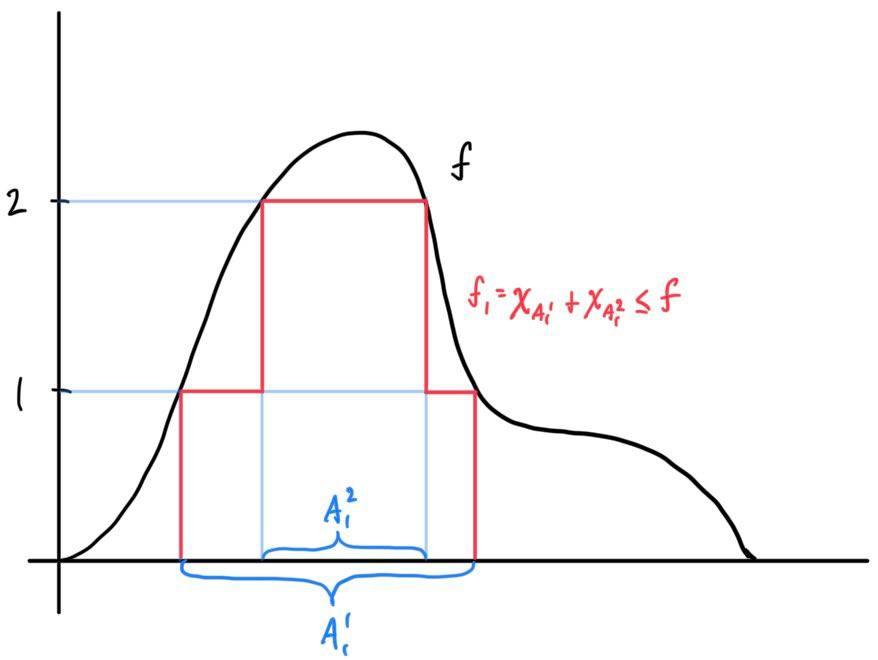
\includegraphics[scale=0.23]{img/Lebesgue_1.jpg}
    \end{center}
    Doing this again with finer subintervals of the codomain gives us, with $f_2 = \chi_{A_2^1} + \chi_{A_2^2} + \chi_{A_2^3} + \chi_{A_2^4} \leq f$. 
    \begin{center}
      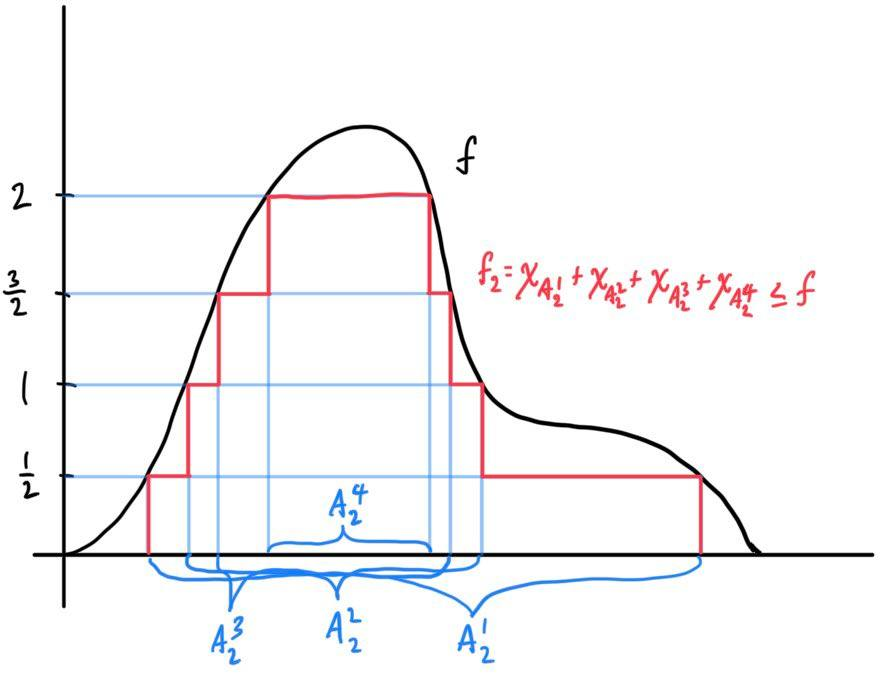
\includegraphics[scale=0.23]{img/Lebesgue_2.jpg}
    \end{center}
    and in general, we have $f_k = \sum_{j=1}^\infty \frac{1}{2^{k-1}} \chi_{A^j_k}$. But we said a simple function is a \textit{finite} sum, and if $\infty$ is in the range of $f$, then this becomes a problem. We can quickly fix this by just truncating the summation at a certain point in the codomain ($f_1$ only considers intervals up to $1$, $f_2$ up to $2$ and so on), ultimately giving us 
    \begin{equation}
      f_k = \sum_{j=1}^{k 2^{k-1}} \frac{1}{2^{k-1}} \chi_{A^j_k} 
    \end{equation}
  \end{proof}

